\chapter{Results} %rename to results and discussion
\label{ch_results}

%todo: remove this
%%%%%%%%%%	DISCUSSION	%%%%%%%%%%
%\textbf{Discussion}\\

%%%%%%%%%%	/DISCUSSION	%%%%%%%%%%

%%%%%%%%%%%%%%%%%%%%%%%%%%%%%%%%%%%%%%%%%%%
%%%%%%%%%%%%%%%%%%%%%%%%%%%%%%%%%%%%%%%%%%%



\section{Module Evaluation}

\subsection{Carrier Waveform Generation Performance}

Figure \ref{fig:carrier_steady_state} shows the steady state output of the carrier waveform generation module (blue trace) for a constant high logic level at the input (red trace). The frequency of the output waveform was calculated to be 40.2kHz.

\begin{figure}[H]
	\centering
	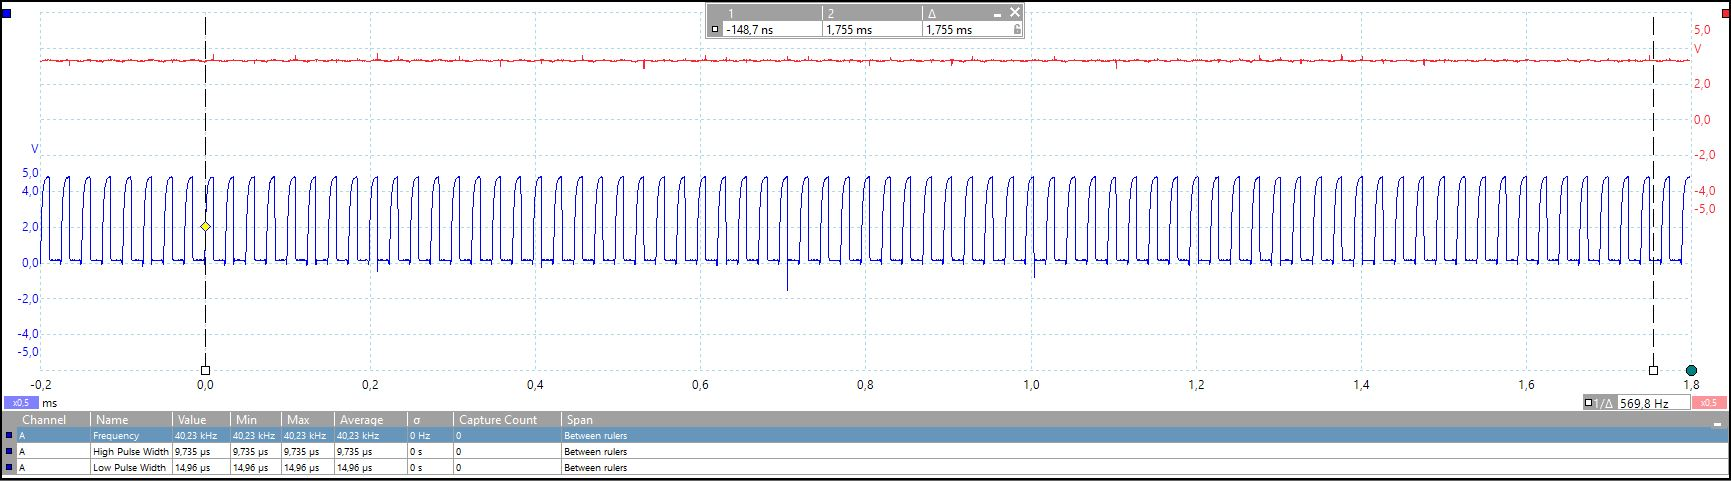
\includegraphics[width=.9\linewidth]{figures/results/carrier_waveform_generation/steady_state.JPG}
	\captionof{figure}{Carrier Generation - Constant Generation}
	\label{fig:carrier_steady_state}
\end{figure}

Figure \ref{fig:carrier_manchester_zoomed_view} presents a zoomed in view of a Manchester transmission (red trace) at the input of the carrier waveform generation module and the corresponding output waveform (blue trace). The frequency of the carrier generated in these short bursts was measured to be 38.4kHz.

\begin{figure}[H]
	\centering
	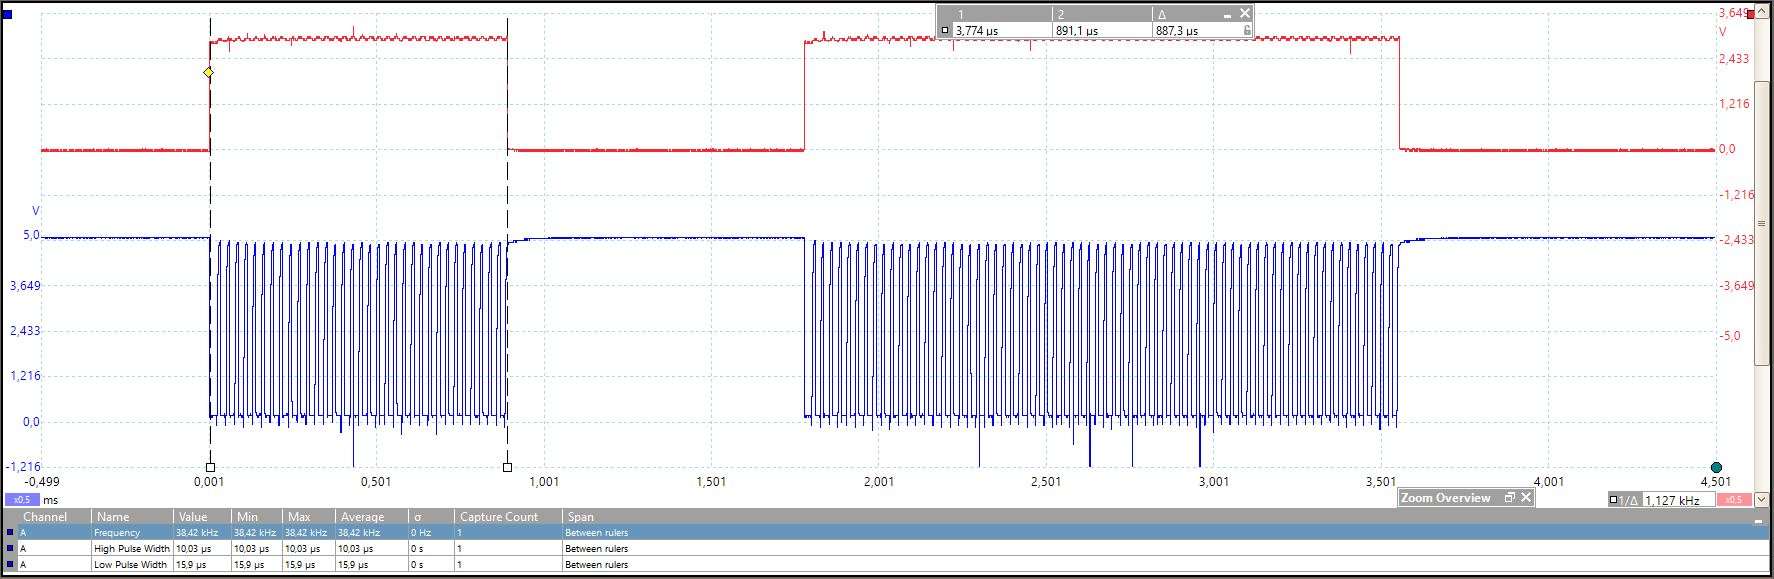
\includegraphics[width=.9\linewidth]{figures/results/carrier_waveform_generation/manchester_zoomed_view.JPG}
	\captionof{figure}{Manchester Transmission - Carrier Inspection}
	\label{fig:carrier_manchester_zoomed_view}
\end{figure}

In both cases, the duty cycle of the carrier waveform was 39\%.


%%%%%%%%%%	DISCUSSION	%%%%%%%%%%
\textbf{Discussion}\\
The 1.8kHz difference in tone frequency under different modes of operation might be as a consequence of the IC heating up during operation. It was observed that the temperature of the IC increased during prolonged operation.

The measured duty cycle is 6\% less than theoretically predicted, this difference is likely a consequence of the resistor tolerances, as the duty cycle depends only on the external resistors.

The duty cycle remaining the same for both modes of operation supports the hypothesis that the difference in frequency is due to an internal factor such as temperature.
%%%%%%%%%%	/DISCUSSION	%%%%%%%%%%


%%%%%%%%%%%%%%%%%%%%%%%%%%%%%%%%%%%%%%%%%%%




\subsection{Power LED Driver Performance}

The following screenshots shown in figures \ref{fig:pwr_led_6k} through \ref{fig:pwr_led_96k} show the results captured by the oscilloscope. The red trace shows the output of the function generator and the blue trace shows the voltage across the shunt resistor R1\footnote{see schematic in figure \ref{fig:schematic_power_led_driver}}.

\begin{figure}[H]
	\centering
	\begin{minipage}{.399\linewidth}
		\centering
		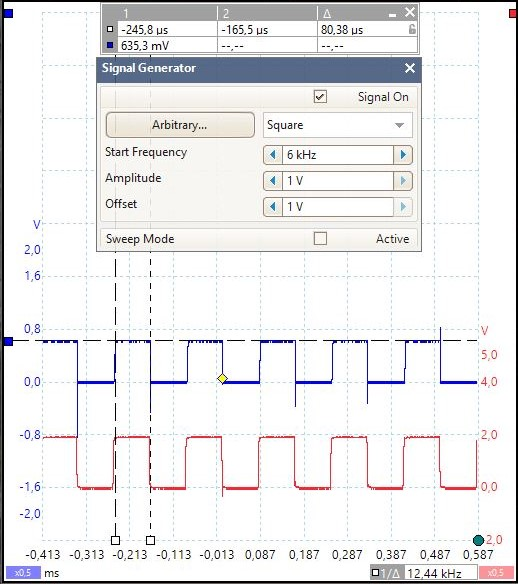
\includegraphics[width=\textwidth]{figures/results/power_led_driver/6khz_crop.JPG}
		\captionof{figure}{6kHz Driving Frequency}
		\label{fig:pwr_led_6k}
	\end{minipage}%
	\hspace{.1\linewidth}
	\begin{minipage}{.399\linewidth}
		\centering
		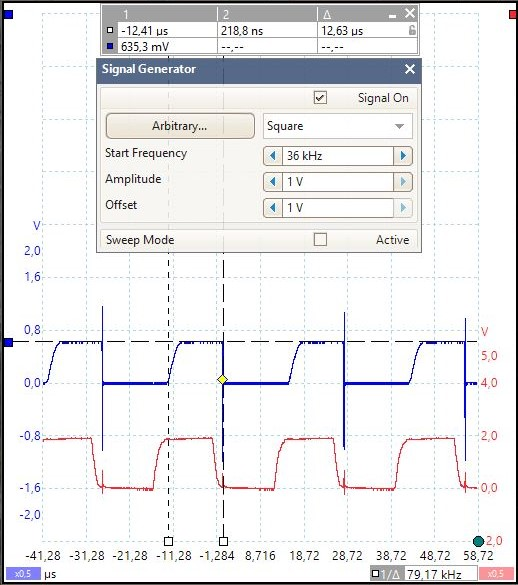
\includegraphics[width=\textwidth]{figures/results/power_led_driver/36khz_crop.JPG}
		\captionof{figure}{36kHz Driving Frequency}
		\label{fig:pwr_led_36k}
	\end{minipage}
\end{figure}

\begin{figure}[H]
	\centering
	\begin{minipage}{.4\linewidth}
		\centering
		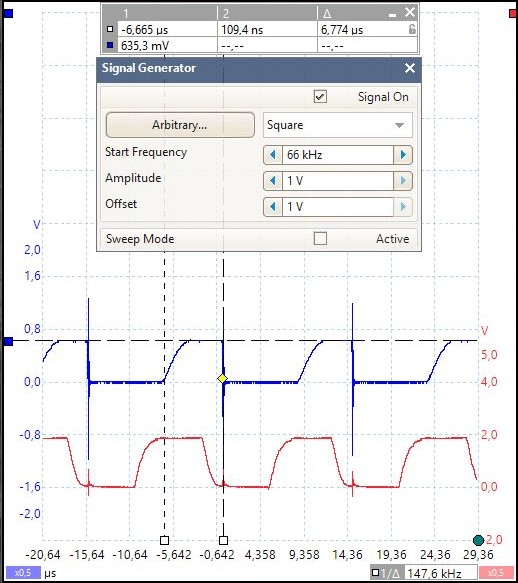
\includegraphics[width=\textwidth]{figures/results/power_led_driver/66khz_crop.JPG}
		\captionof{figure}{66kHz Driving Frequency}
		\label{fig:pwr_led_66k}
	\end{minipage}
	\hspace{.1\linewidth}
	\begin{minipage}{.4\linewidth}
		\centering
		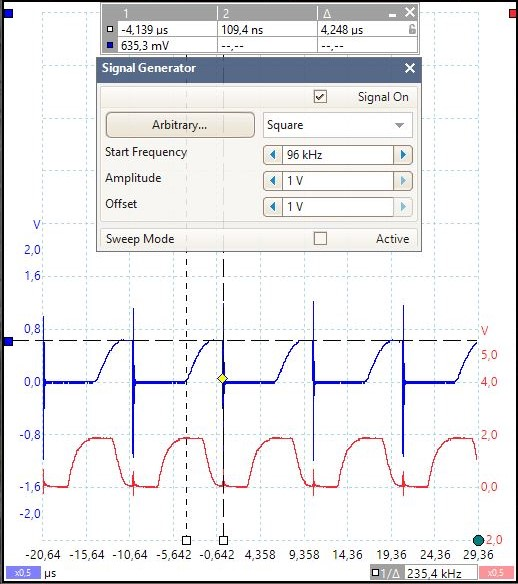
\includegraphics[width=\textwidth]{figures/results/power_led_driver/96khz_crop.JPG}
		\captionof{figure}{96kHz Driving Frequency}
		\label{fig:pwr_led_96k}
	\end{minipage}
\end{figure}

\begin{table}[H]
	\centering
	\begin{tabular}{ccc}
		\hline
		\textbf{\begin{tabular}[c]{@{}c@{}}Frequency\\ (kHz)\end{tabular}} & \textbf{\begin{tabular}[c]{@{}c@{}}LED Current\\ (mA)\end{tabular}} & \textbf{\begin{tabular}[c]{@{}c@{}}Duty Cycle\\ (\%)\end{tabular}} \\ \hline
		6 & 908 & 48.2 \\ \hline
		36 & 908 & 45.5 \\ \hline
		66 & 908 & 44.7 \\ \hline
		96 & 908 & 40.8 \\ \hline
	\end{tabular}
	\caption{Frequency V.S. Current and Pulse Width}
	\label{tbl:led_driver_tabulated_results}
\end{table}


%%%%%%%%%%	DISCUSSION	%%%%%%%%%%
\textbf{Discussion}\\
For each test frequency, the power LED driver module regulated the current with a high precision and no noticeable ripple. This encapsulates the advantages of linear regulation.

The design predicted a current limit of 1.02A. These results show that the real current limit is 0.91A. This result predicts that the actual base-emitter voltage drop\footnote{at equilibrium} is closer to 0.62V.

The duty cycle of the LED current decreases for increasing input frequencies. This can be attributed to the rise-time of the current through the LED (the time taken for the current to reach steady state). As the driving frequency increases, this rise-time makes up an increasing portion of the total on-time.
%%%%%%%%%%	/DISCUSSION	%%%%%%%%%%


%%%%%%%%%%%%%%%%%%%%%%%%%%%%%%%%%%%%%%%%%%%





\subsection{Light Focus System}

\subsubsection{Focal Length of Lens}

The measured focal length of the lens was measured to be 53mm. Figure \ref{fig:focal_length_experiemnt_result} shows the focused point formed after adjusting the lens to 5.3cm above the working surface.

\begin{figure}[H]
	\centering
	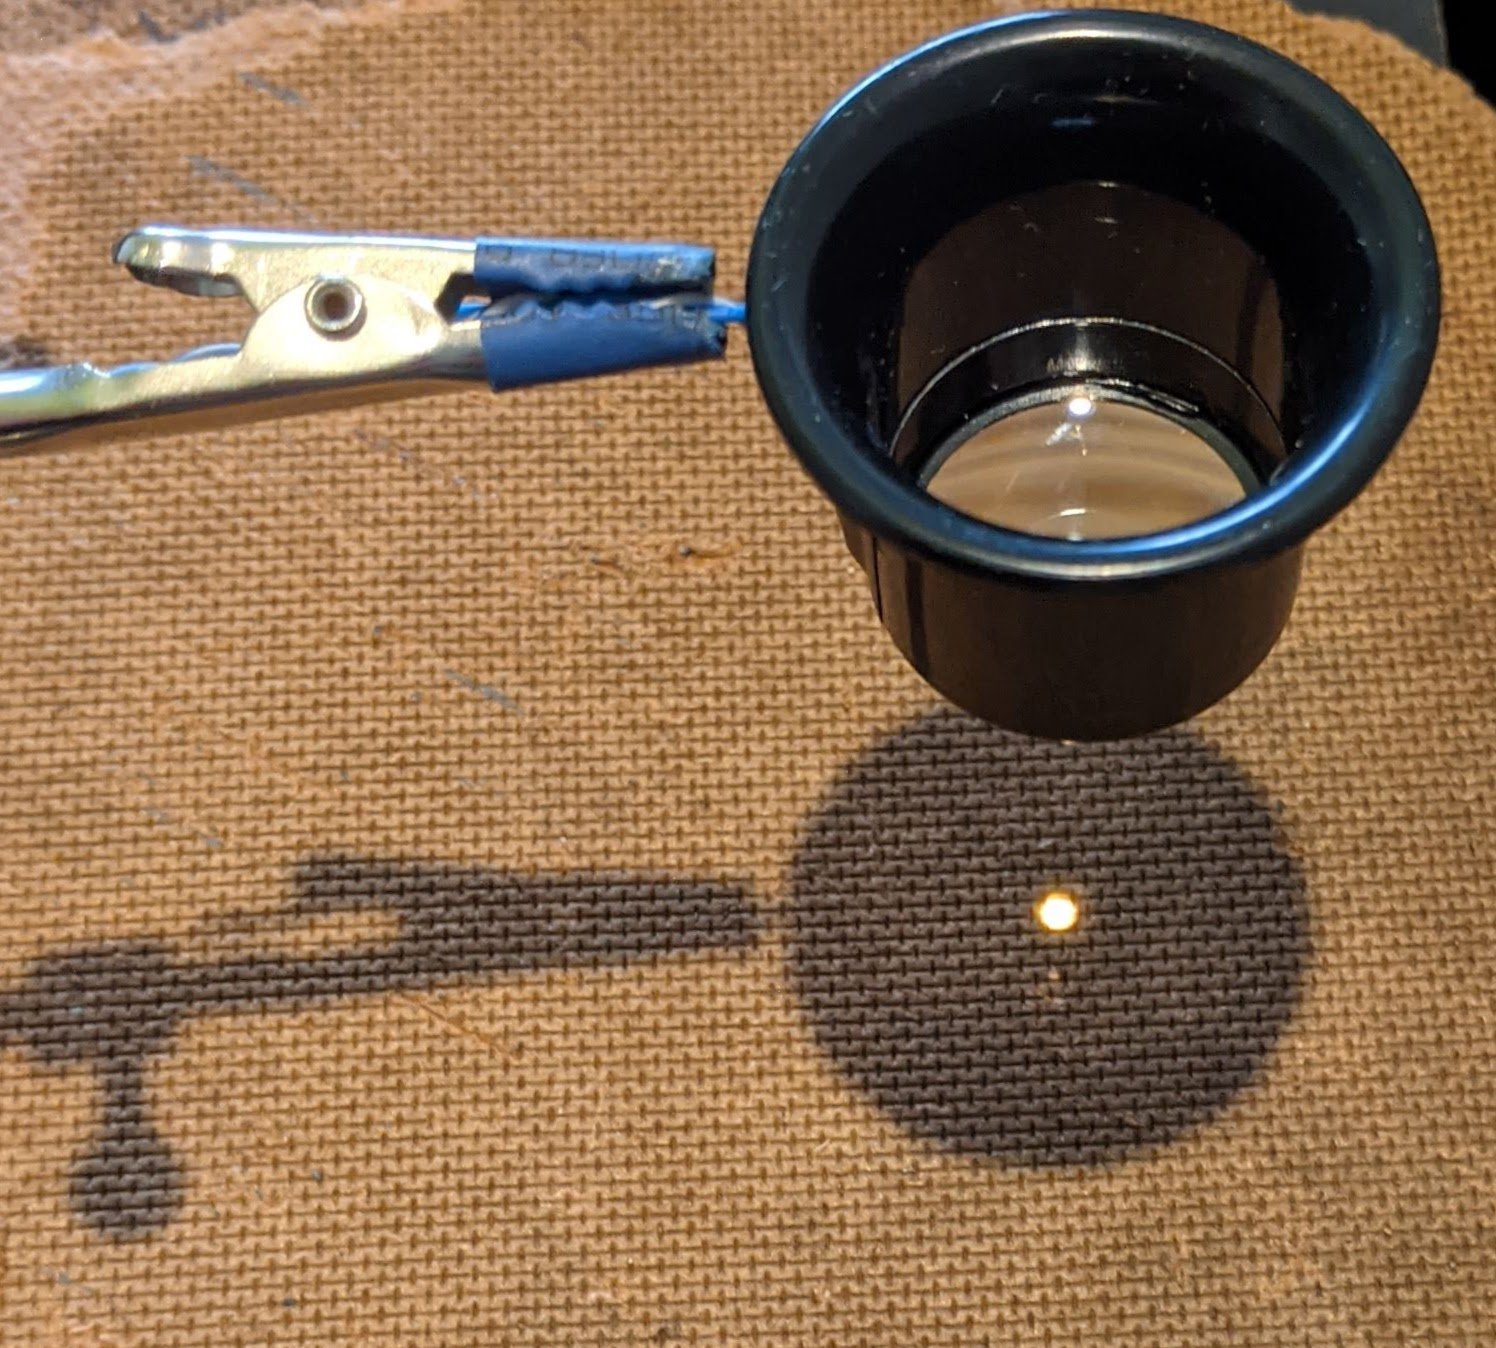
\includegraphics[width=.6\linewidth]{figures/results/focal_length_result.jpg}
	\captionof{figure}{Focal Length Experiemnt}
	\label{fig:focal_length_experiemnt_result}
\end{figure}


\subsubsection{IR Beam Dispersion}

\begin{figure}[H]
	\centering
	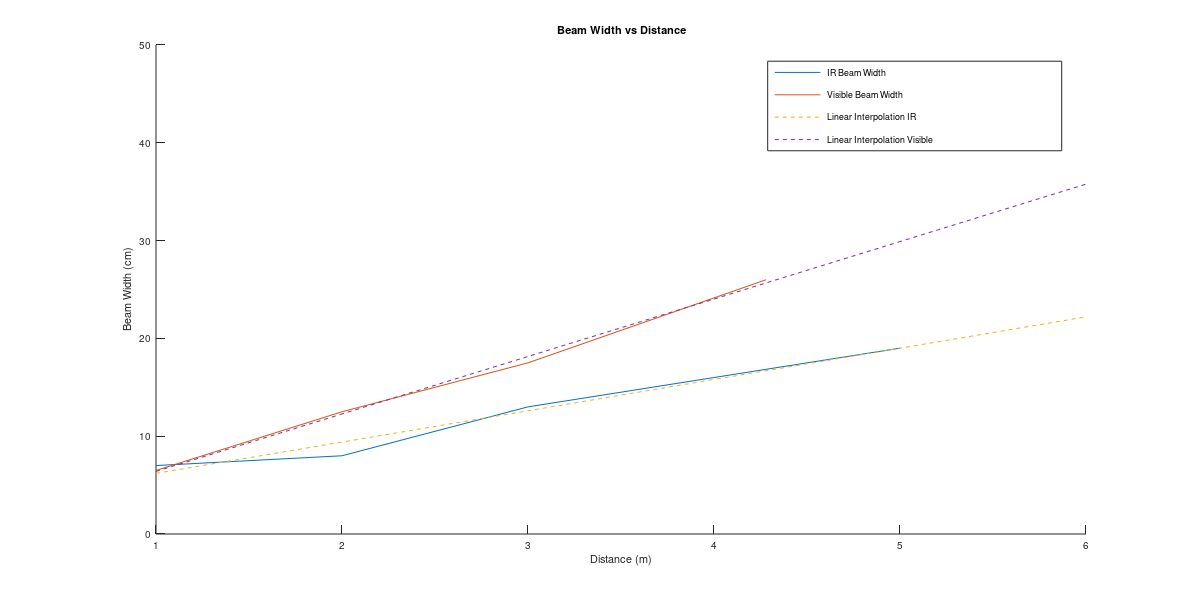
\includegraphics[width=\linewidth]{figures/results/beam_width_vs_distance.png}
	\captionof{figure}{Beam Width vs Distance}
	\label{fig:beam_width_vs_distance}
\end{figure}



%todo: ref this table
Table \ref{tbl:spot_size_vs_distance} below shows the beam spot size vs distance for the IR and white power LEDs.

%todo: update these images
\begin{figure}[H]
	\centering
	\begin{minipage}{.4\textwidth}
		%todo: make image higher quality after zoom
		\textbf{Linear Interpolation Equations}
		
		\[width_{ir\: beam} = 0.03 + 0.032 \times d_{beam}\]
		
		\[width_{visible\: beam} = 0.00526 + 0.0587 \times d_{beam}\]
		
		
	\end{minipage}%
	\hspace{.1\textwidth}
	\begin{minipage}{.4\textwidth}
		\begin{table}[H]
			\begin{tabular}{ccc}
				\hline
				\textbf{\begin{tabular}[c]{@{}c@{}}Distance\\ (m)\end{tabular}} & \textbf{\begin{tabular}[c]{@{}c@{}}IR Beam\\ Width\\ (cm)\end{tabular}} & \textbf{\begin{tabular}[c]{@{}c@{}}Visible Beam\\ Width\\ (cm)\end{tabular}} \\ \hline
				1 & 7 & 6.5 \\ \hline
				2 & 8 & 12.5 \\ \hline
				3 & 13 & 17.5 \\ \hline
				4 & 16 & - \\ \hline
				4.28 & - & 26 \\ \hline
				5 & 19 & - \\ \hline
			\end{tabular}
			\captionof{table}{Tabulation of Spot Diameter V.S. Distance}
			\label{tbl:spot_size_vs_distance}
		\end{table}
	\end{minipage}
\end{figure}

%todo: comment on the observation of the led 'square' pattern.

%%%%%%%%%%	DISCUSSION	%%%%%%%%%%
\textbf{Discussion}\\
%todo: discuss these results
%%%%%%%%%%	/DISCUSSION	%%%%%%%%%%


%%%%%%%%%%%%%%%%%%%%%%%%%%%%%%%%%%%%%%%%%%%




\subsection{Directivity of IR Modules}

Figure \ref{fig:vrms_vs_angle_of_incidence} shows the RMS voltage value of the modules output with respect to the angle of incidence. Figure \ref{fig:beam_pattern} shows the normalized RMS voltage value and mirrors the image about the vertical to provide an illustration of the beam pattern.


\begin{figure}[H]
	\centering
	\begin{minipage}{.4\linewidth}
		\centering
		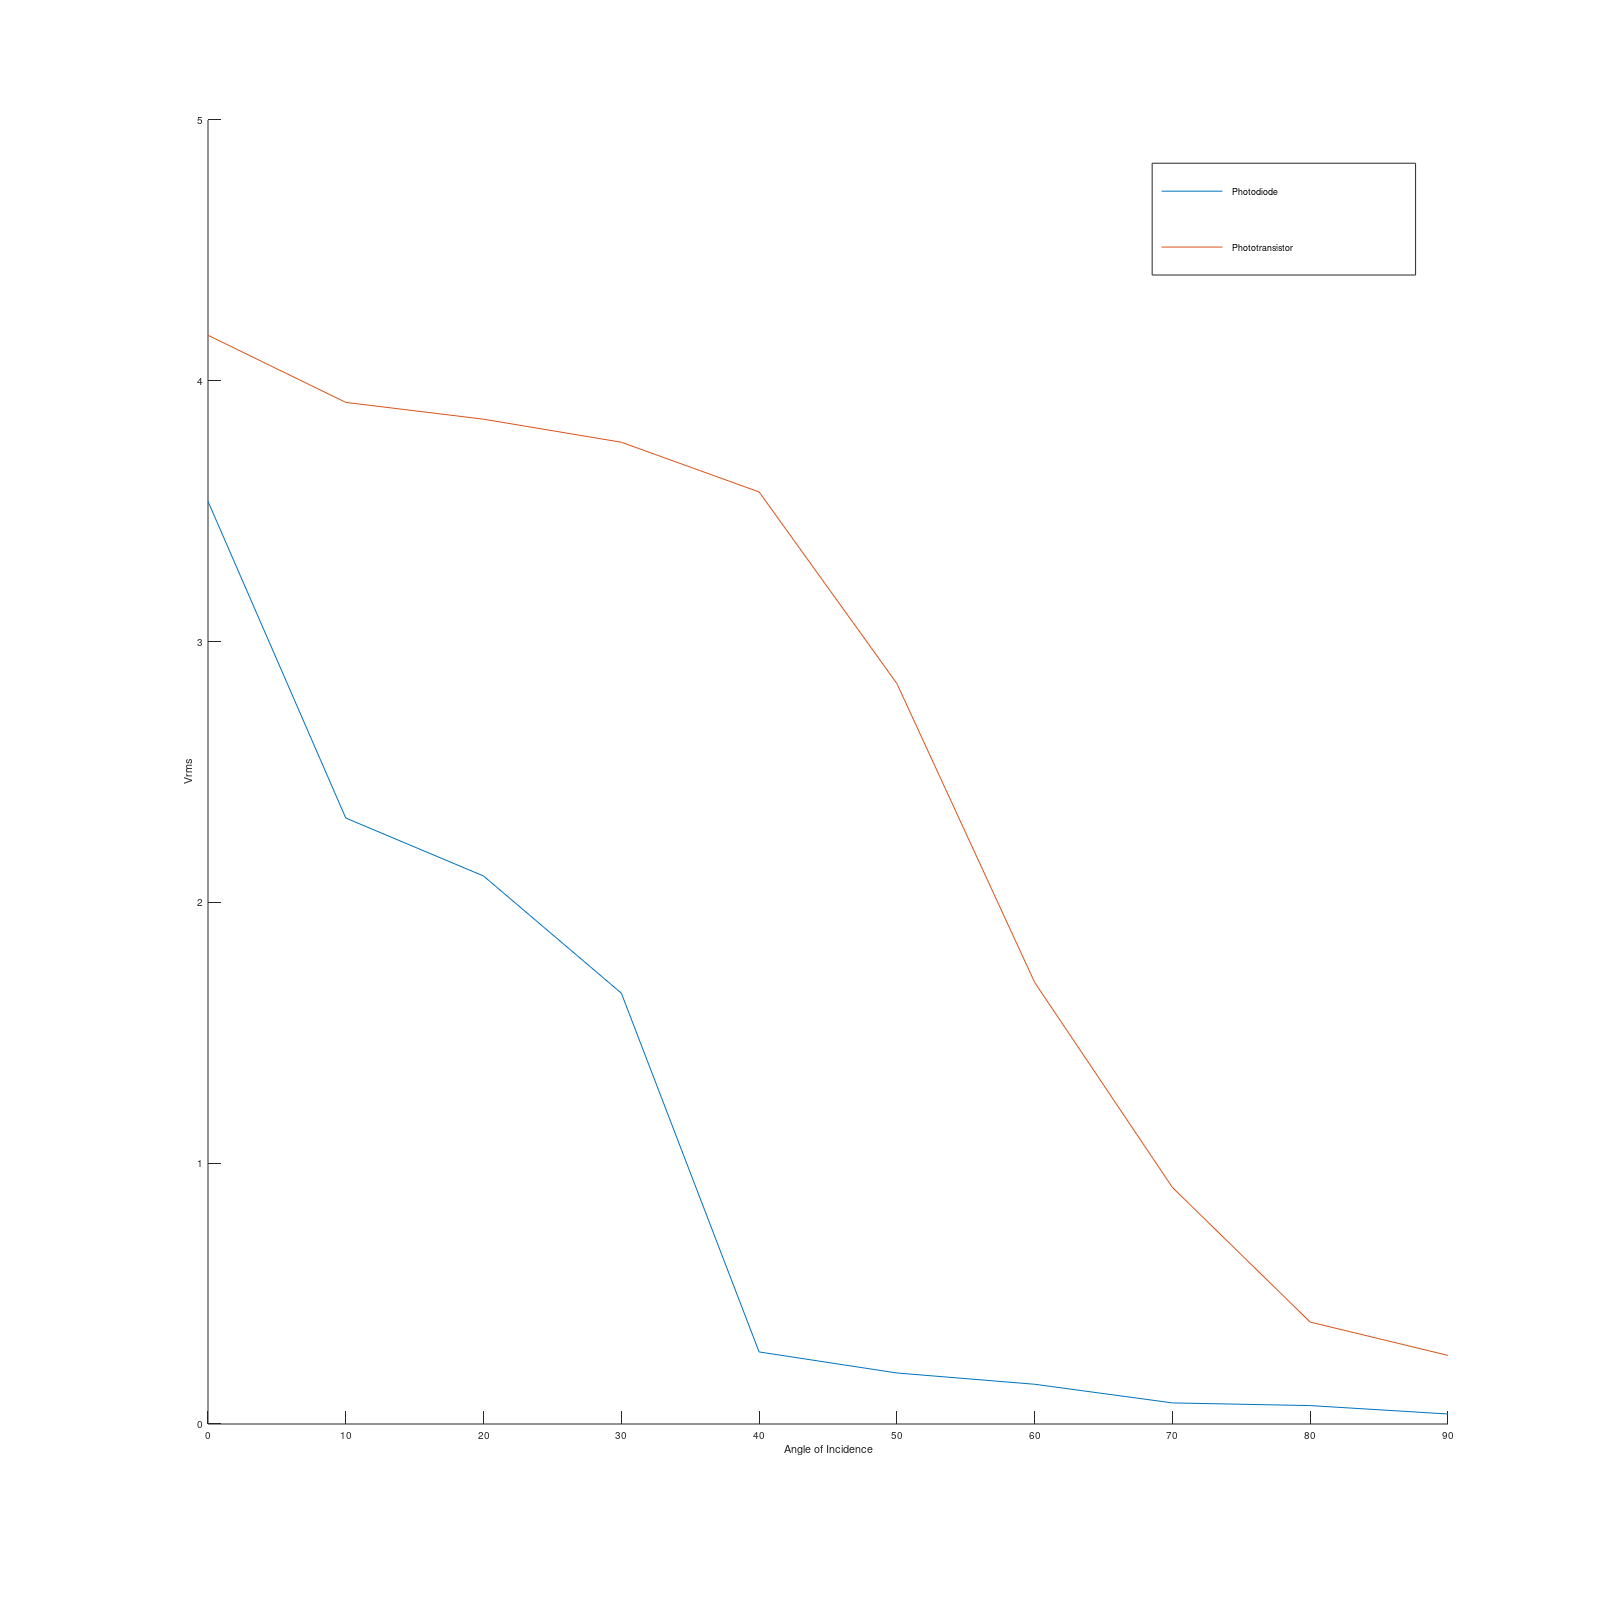
\includegraphics[width=\textwidth]{figures/results/vrms_vs_incidence_square.png}
		\captionof{figure}{Vrms vs Angle of Incidence}
		\label{fig:vrms_vs_angle_of_incidence}
	\end{minipage}
	\hspace{.1\linewidth}
	\begin{minipage}{.4\linewidth}
		\centering
		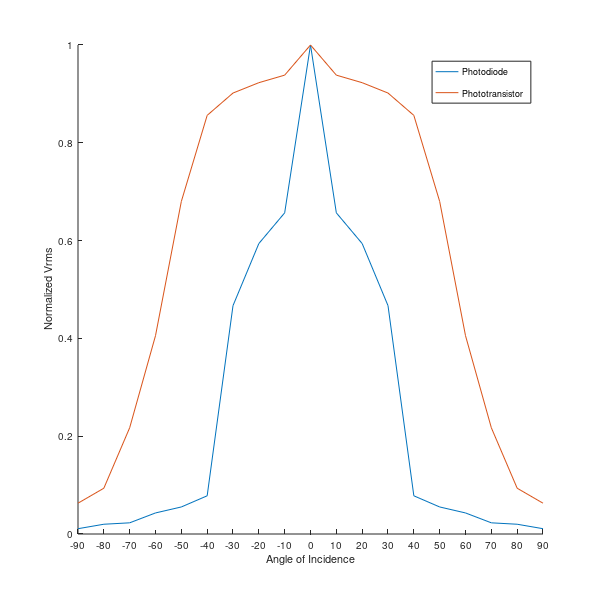
\includegraphics[width=\textwidth]{figures/results/beam_pattern_square.png}
		\captionof{figure}{Beam Pattern}
		\label{fig:beam_pattern}
	\end{minipage}
\end{figure}

The IR receiver module registered the signal between angles of 0\textdegree and 70\textdegree and registered an absence of a signal for angles greater than 80\textdegree. Between 70\textdegree and 80\textdegree the output would toggle sporadically.


%%%%%%%%%%	DISCUSSION	%%%%%%%%%%
\textbf{Discussion}\\
%todo: discuss these results
%%%%%%%%%%	/DISCUSSION	%%%%%%%%%%




%%%%%%%%%%%%%%%%%%%%%%%%%%%%%%%%%%%%%%%%%%%




\subsection{Signal Conditioning Performance}

\subsubsection{Anti-alias Filtering}
Figure \ref{fig:anti_alias_filtering} below shows the oscilloscope trace of the 36kHz square waveform being generated at the input to the signal conditioning module (blue) and the filtered output waveform (red).

\begin{figure}[H]
	\centering
	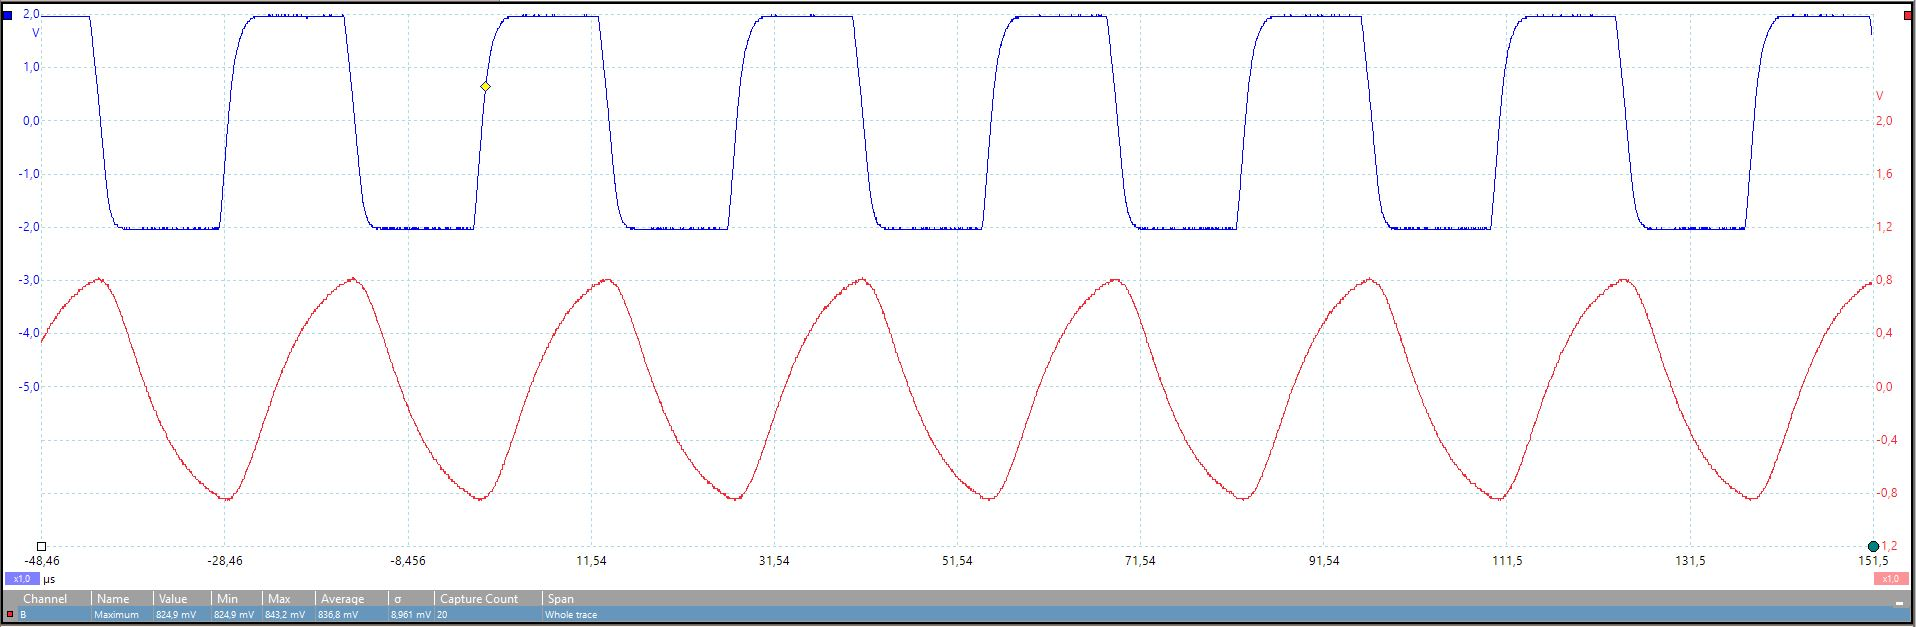
\includegraphics[width=\textwidth]{figures/results/low_pass_filter/36kHzsquarewavein.JPG}
	\captionof{figure}{Osciliscope output showing signal before and after filtering}
	\label{fig:anti_alias_filtering}
\end{figure}

%%%%%%%%%%	DISCUSSION	%%%%%%%%%%
%comment: this is lame but not much else to say...
\textbf{Discussion}\\
Visual inspection confirms that the anti-alias filter is removing the higher frequency components. The amplitude of the output waveform is less than half the amplitude of the input waveform, this reduction is mostly as a consequence of the voltage divider at the filter's input.
%%%%%%%%%%	/DISCUSSION	%%%%%%%%%%

\subsubsection{Precision Rectification}

Figure \ref{fig:precision_rectification} below shows the oscilloscope trace of the signal being fed into the precision rectifier (blue) and the resulting rectified signal (red).

\begin{figure}[H]
	\centering
	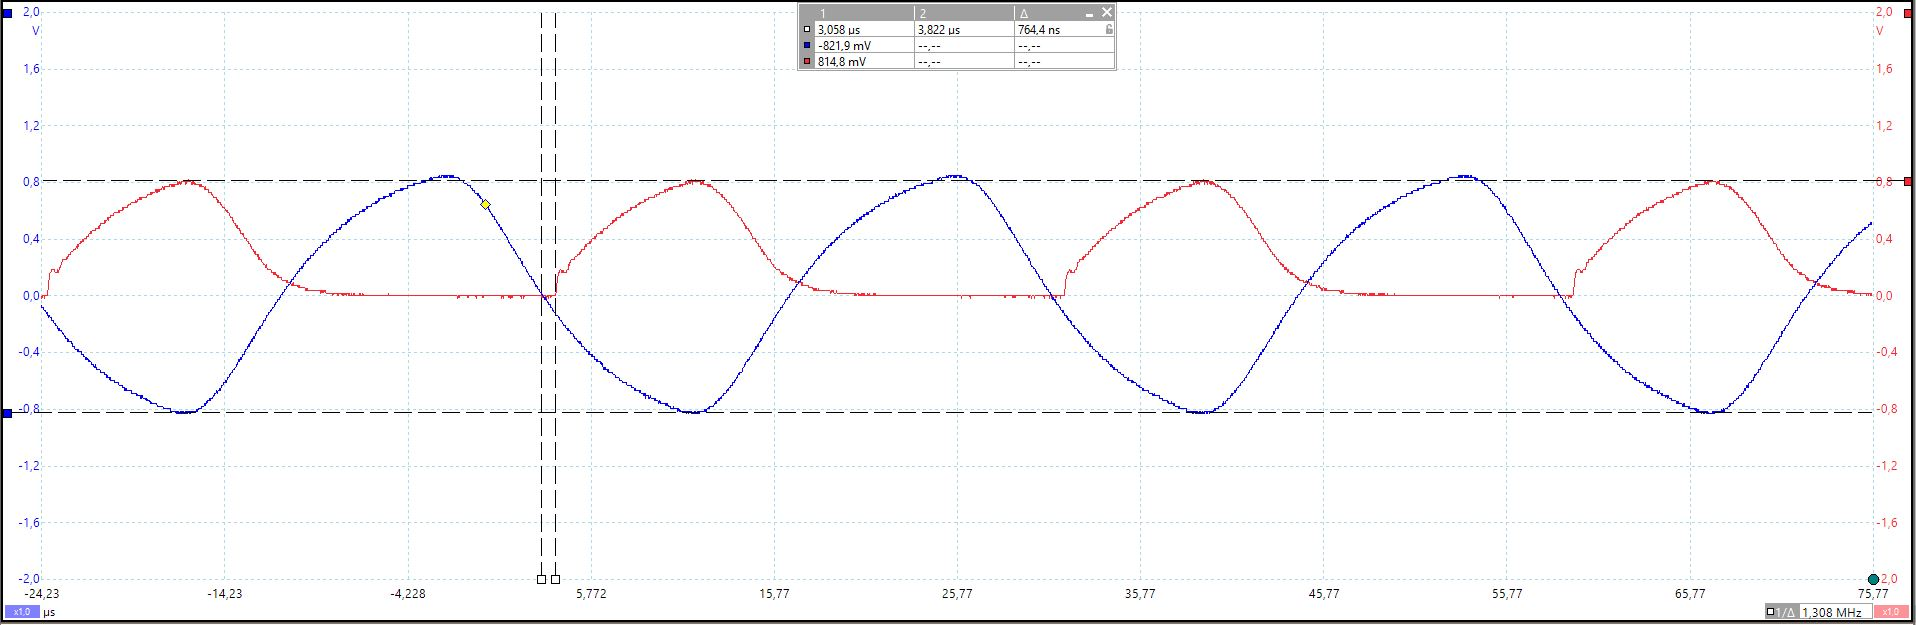
\includegraphics[width=\textwidth]{figures/results/rectification/36kHz.JPG}
	\captionof{figure}{Osciliscope output showing signal before and after rectification}
	\label{fig:precision_rectification}
\end{figure}

%%%%%%%%%%	DISCUSSION	%%%%%%%%%%
\textbf{Discussion}\\
The precision rectifier stage operates as expected, the difference between the amplitude of the input signal and output signal during rectification is 7mV.

A 765ns cross-over delay can be observed, this is the period of time that elapses between the instant the blue signal becomes negative and the instant the red signal starts to rise. This occurs because the op-amp requires a finite period of time to swing the output voltage such that it exceeds the forward voltages of the two diodes.
%%%%%%%%%%	/DISCUSSION	%%%%%%%%%%




%%%%%%%%%%%%%%%%%%%%%%%%%%%%%%%%%%%%%%%%%%%




\subsection{Goertzel Filter Performance}

\subsubsection{Simulated Frequency Response}

\begin{figure}[H]
	\centering
	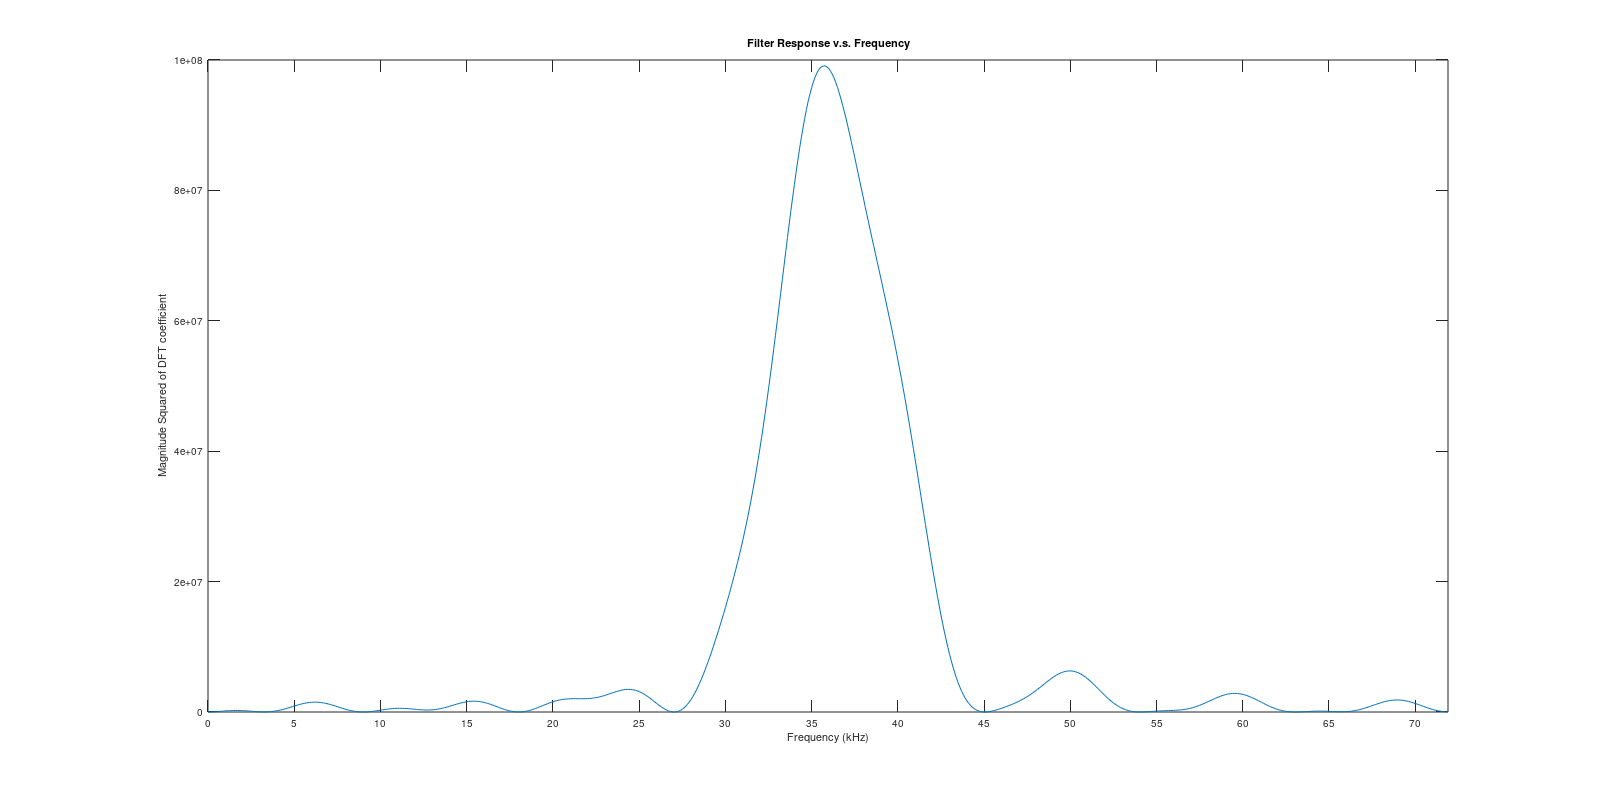
\includegraphics[width=\linewidth]{figures/results/goertzel_filter_simulation_wide.png}
	\caption{Expected Frequency Response - Goertzel Filter}
	\label{fig:goertzel_filter_response_simulated}
\end{figure}



%%%%%%%%%%	DISCUSSION	%%%%%%%%%%
\textbf{Discussion}\\
The simulation results shown in figure \ref{fig:goertzel_filter_response_simulated} reveal the familiar sinc function embedded in the frequency response curves. The form of these curves can be characterised by the $sinc^2(x)$ function which is to be expected because the filter returns the square of the magnitude.

It is clear from the plot that the filter is highly sensitive to the magnitude of the sampled waveform. A decrease in amplitude by a factor of two results in a four fold decrease in the amplitude of the filters response.
%%%%%%%%%%	/DISCUSSION	%%%%%%%%%%




\subsubsection{Measured Frequency Response}

The following plot in figure \ref{fig:goertzel_filter_response_empirical} show the values returned by the Goertzel filter module and shows the expected frequency response curve.

\begin{figure}[H]
	\centering
	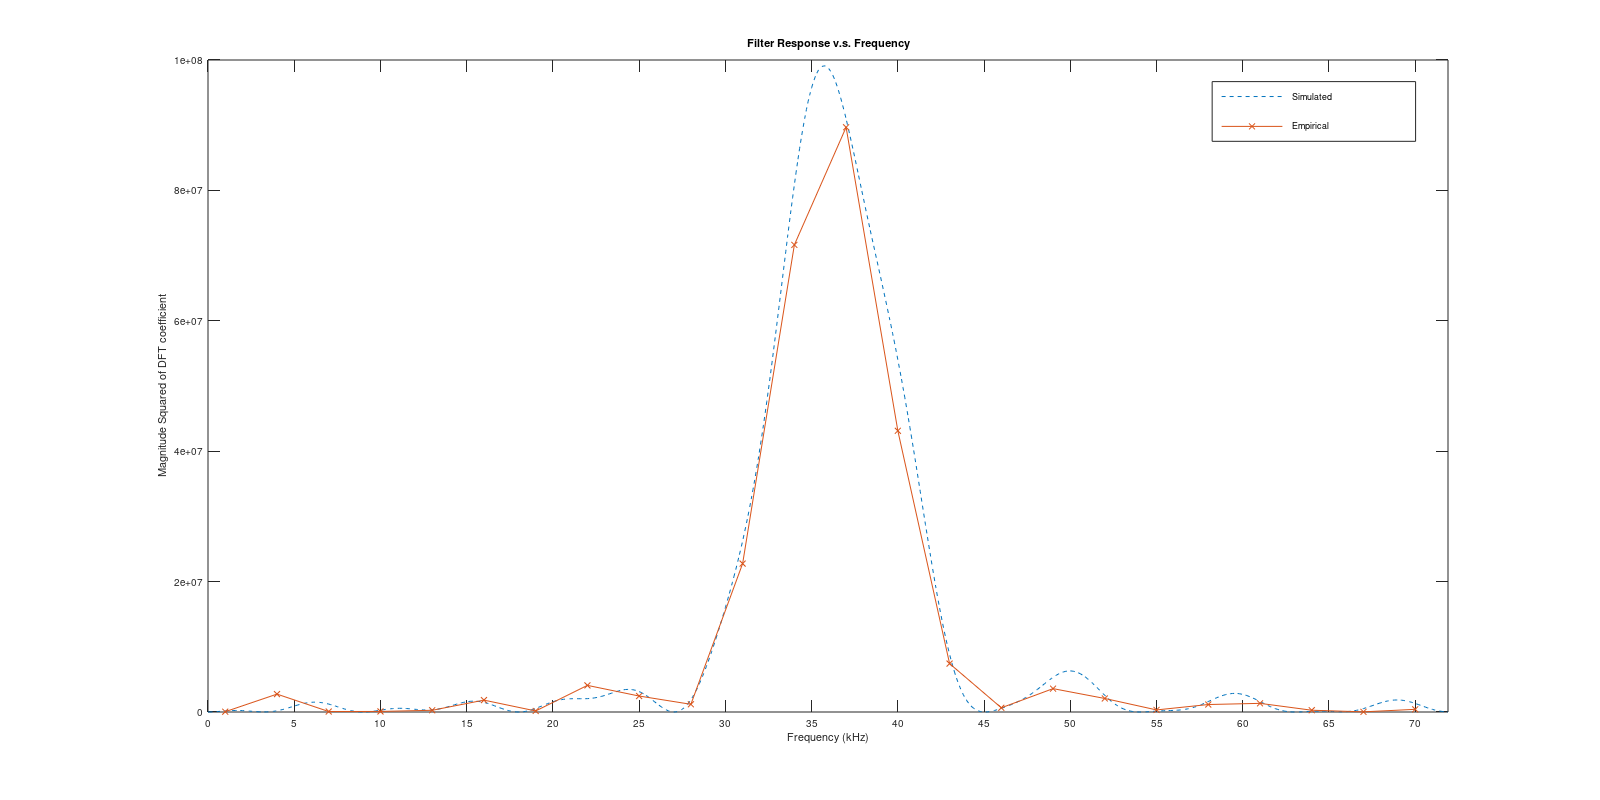
\includegraphics[width=\linewidth]{figures/results/goertzel_filter_empirical_wide.png}
	\caption{Measured Frequency Response - Goertzel Filter}
	\label{fig:goertzel_filter_response_empirical}
\end{figure}


%%%%%%%%%%	DISCUSSION	%%%%%%%%%%
\textbf{Discussion}\\
%todo: discuss these results
%%%%%%%%%%	/DISCUSSION	%%%%%%%%%%




\subsubsection{Trigger Conditions}

\begin{table}[H]
	\centering
	\begin{tabular}{ccc}
		\hline
		\begin{tabular}[c]{@{}c@{}}Amplitude\\ (mV)\end{tabular} & \begin{tabular}[c]{@{}c@{}}Trigger Frequency\\ Lower (kHz)\end{tabular} & \begin{tabular}[c]{@{}c@{}}Trigger Frequency\\ Upper (kHz)\end{tabular} \\ \hline
		297 & 35.12 & 36.79 \\ \hline
		300 & 34.7 & 37.23 \\ \hline
		350 & 32.74 & 39.27 \\ \hline
		400 & 31.86 & 40.16 \\ \hline
		450 & 31.29 & 40.78 \\ \hline
		500 & 30.86 & 41.2 \\ \hline
	\end{tabular}
	\captionof{table}{Amplitude-Voltage Boundry Pairs}
	\label{tbl:amplitude_voltage_trigger_pairs}
\end{table}

\begin{figure}[H]
	\centering
	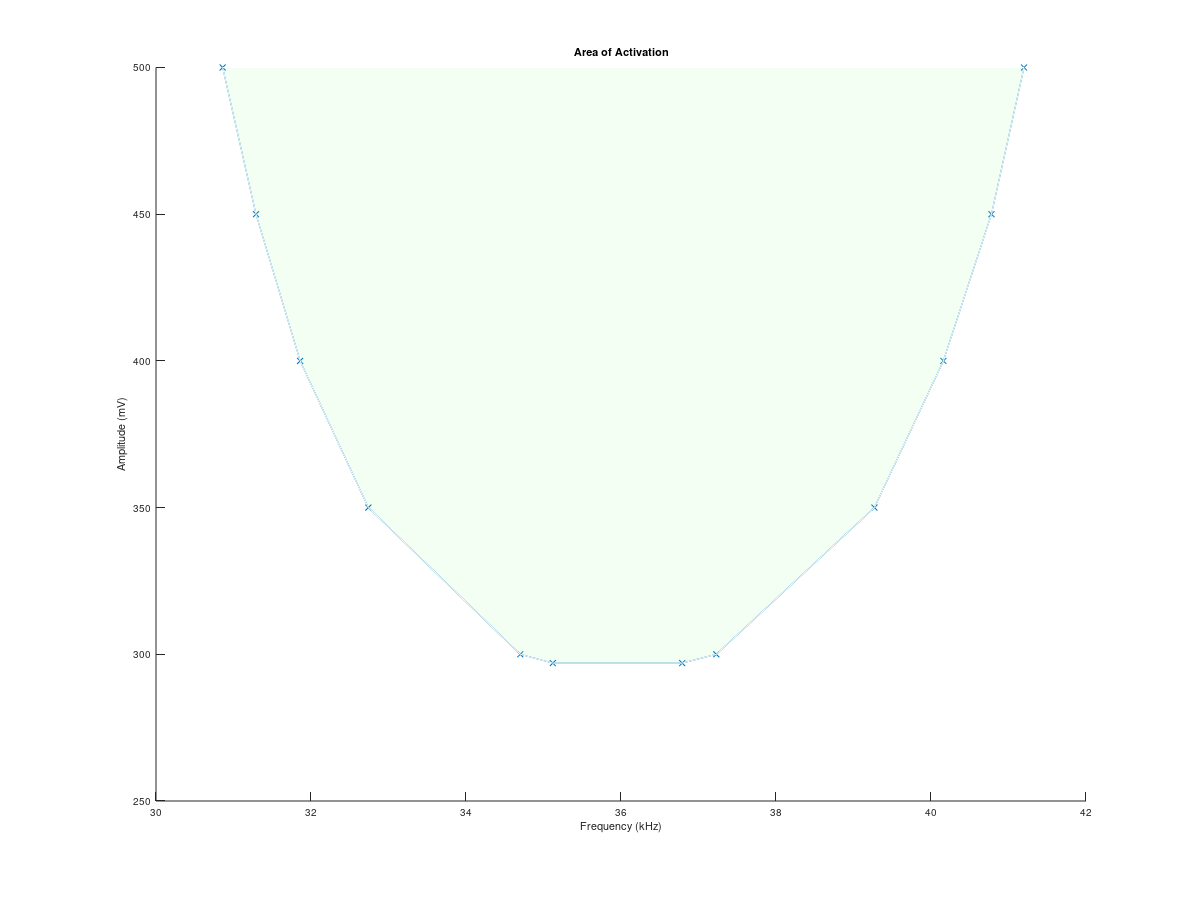
\includegraphics[width=.8\textwidth]{figures/results/goertzel_amplitude_frequency_pairs.png}
	\captionof{figure}{Area of Sensitivity Goertzel Filter}
	\label{fig:goertzel_amplitude_frequency_pairs}
\end{figure}




%%%%%%%%%%	DISCUSSION	%%%%%%%%%%
\textbf{Discussion}\\
%todo: discuss these results
%%%%%%%%%%	/DISCUSSION	%%%%%%%%%%



%%%%%%%%%%%%%%%%%%%%%%%%%%%%%%%%%%%%%%%%%%%



%%%%%%%%%%%%%%%%%%%%%%%%%%%%%%%%%%%%%%%%%%%
%%%%%%%%%%%%%%%%%%%%%%%%%%%%%%%%%%%%%%%%%%%

%%%%%%%%%%%%%%%%%%%%%%%%%%%%%%%%%%%%%%%%%%%
%%%%%%%%%%%%%%%%%%%%%%%%%%%%%%%%%%%%%%%%%%%

\section{Software Evaluation}


\subsection{Goertzel Filter Benchmark}

The results from the goertzel algorithm optimization experiment are tabulated in table \ref{tbl:goertzel_speed_results}, the adjacent screenshot shown in figure \ref{fig:goertzel_speed_scope_screenshot} illustrates the output recorded by the oscilloscope software during a single iteration of the experiment. 

\begin{figure}[H]
	\centering
	\begin{minipage}{.4\textwidth}
		%todo: make image higher quality after zoom
		\centering
		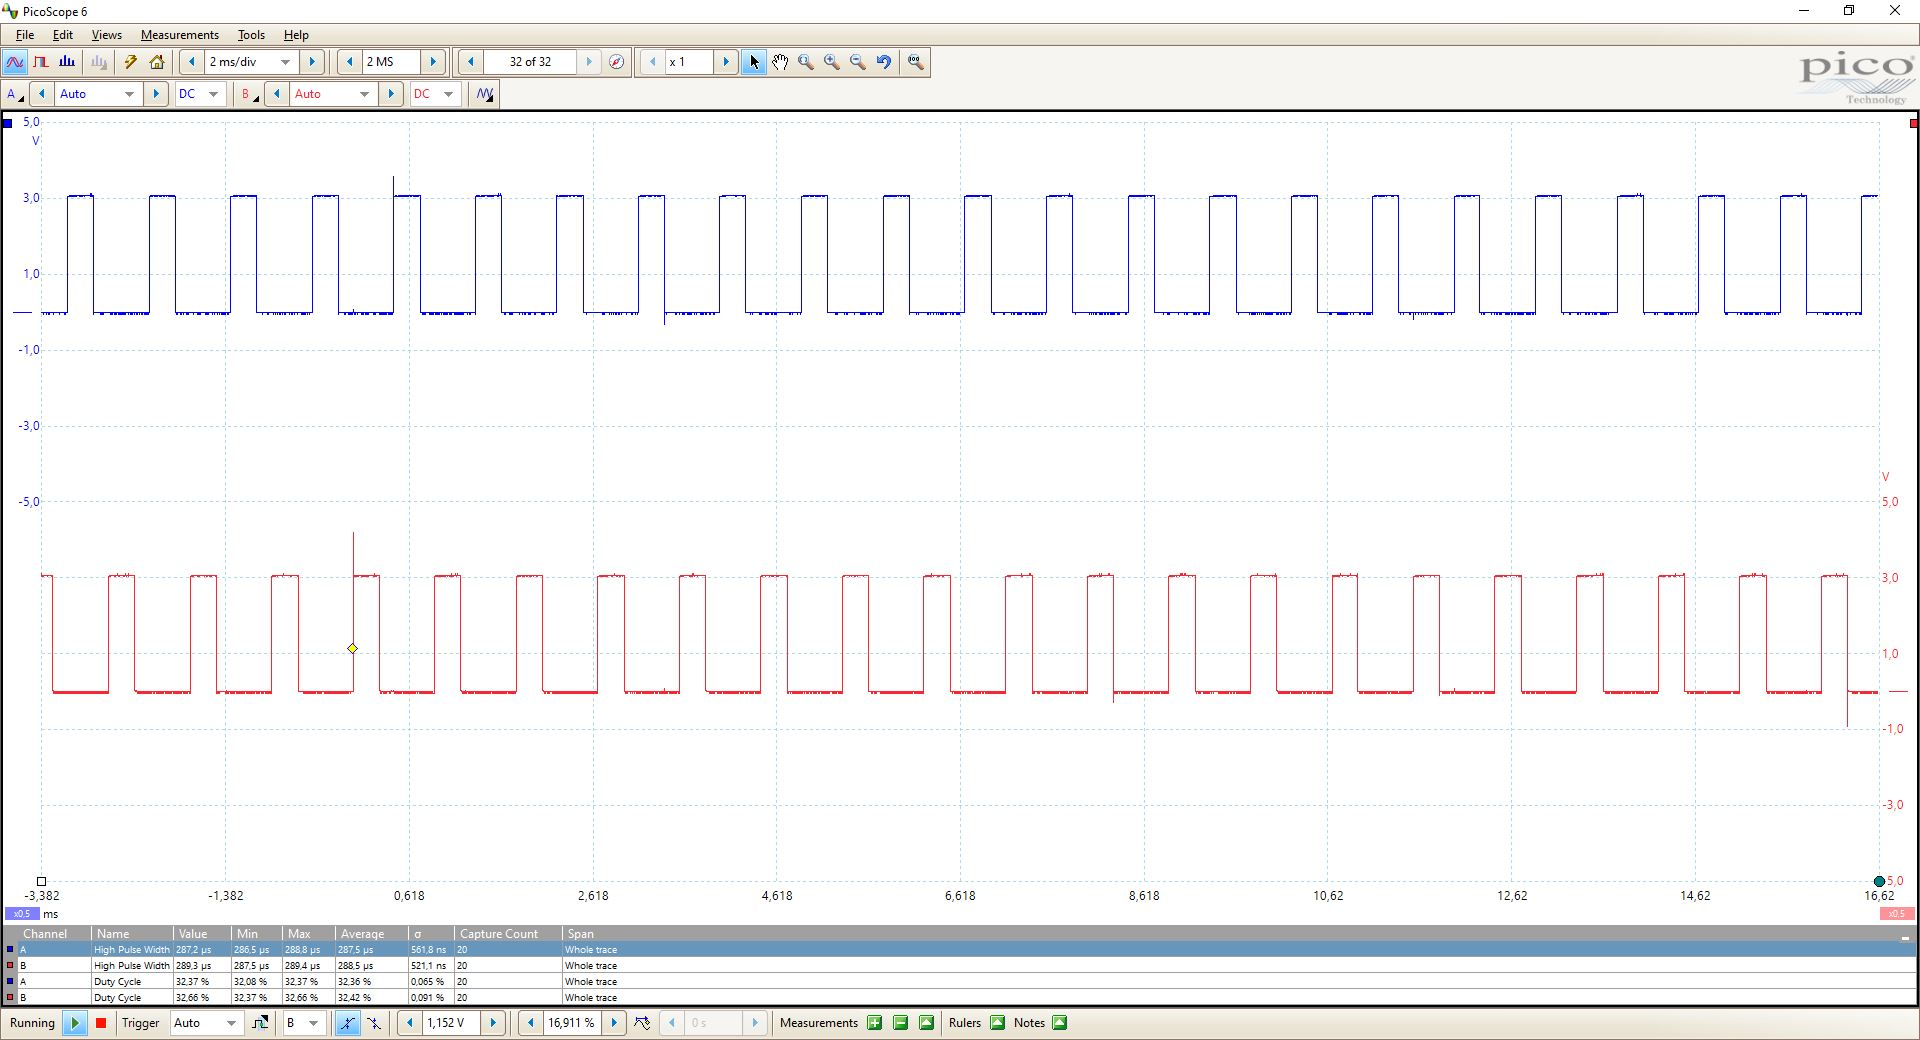
\includegraphics[width=0.9\linewidth]{figures/results/goertzel_filter_speed/16nu.JPG}
		\captionof{figure}{Scope Reading for unoptimized goertzel with $N = 16$}
		\label{fig:goertzel_speed_scope_screenshot}
	\end{minipage}%
	\hspace{.1\textwidth}
	\begin{minipage}{.4\textwidth}
		\begin{table}[H]
			\begin{tabular}{ccc}
				\hline
				\textbf{N} & \textbf{\begin{tabular}[c]{@{}c@{}}Unoptimized\\ ($\mu S$)\end{tabular}} & \textbf{\begin{tabular}[c]{@{}c@{}}Optimized\\ ($\mu S$)\end{tabular}} \\ \hline
				4 & 96.46 & 61.15 \\ \hline
				8 & 160.3 & 98.35 \\ \hline
				16 & 287.5 & 171.9 \\ \hline
				32 & 547.2 & 323.9 \\ \hline
				64 & 1059 & 621.1
			\end{tabular}
			\captionof{table}{Compiled results for goertzel speed experiemnt}
			\label{tbl:goertzel_speed_results}
		\end{table}
	\end{minipage}
\end{figure}

The recorded results are plotted in figure \ref{fig:goertzel_computation_plot} to provide graphical insight.

\begin{figure}[H]
	\centering
	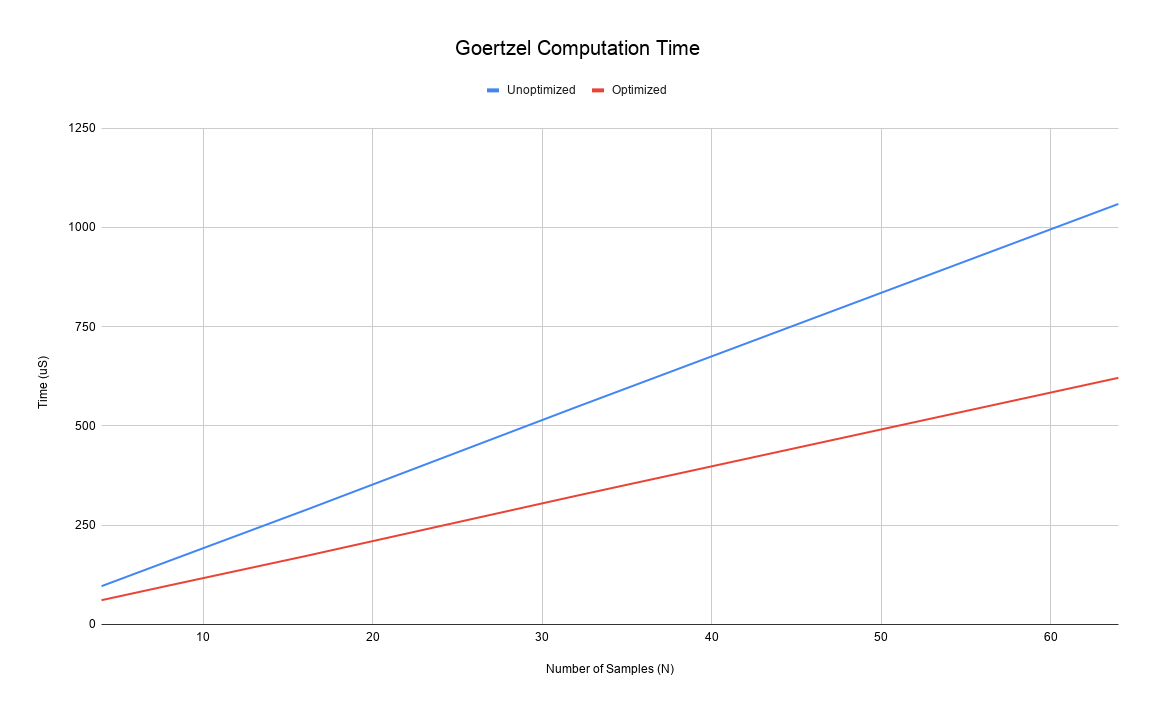
\includegraphics[width=\linewidth]{figures/results/goertzel_filter_speed/goertzel_computation_time.png}
	\captionof{figure}{Goertzel computation time versus sample set size}
	\label{fig:goertzel_computation_plot}
\end{figure}


%%%%%%%%%%	DISCUSSION	%%%%%%%%%%
\textbf{Discussion}\\
Figure \ref{fig:goertzel_computation_plot} provides two important insights to the nature of the goertzel algorithm. The first observation may be found in the linearity of both plots, this confirms that both implementations of the algorithm have a time complexity of O(N) as noted in section \ref{sec:filter_optimization_design}. The practically perfect linearity in the results makes it possible to predict the timing requirements and make accurate theoretical predictions.

The gradient of the unoptimized curve is $16\mu S/sample$ and the gradient of the optimized curve is $9.3\mu S/sample$. The sampling rate used was $f_{sampling} \approx 144$kHz or $6.9\mu S/sample$. This indicates that even after optimizing the algorithm by simplifying out the multiplication step required for each new sample, the processor is still not fast enough to keep up with the rate of incoming samples.

The final observation is that the implemented optimization has two implications for the algorithms performance. The first implication is a small but non-zero constant timer saving, this comes as a result of removing the need for the multiplications to find the real and imaginary components of the k\textsubscript{th} DFT coefficient (see lines 18 and 19 of listing \ref{lst:goertzel_algorithm}). The second implication is a time difference which is directly proportional to the number of samples N, as indicated by the different gradients highlighted in the above paragraph.
%%%%%%%%%%	/DISCUSSION	%%%%%%%%%%


%%%%%%%%%%%%%%%%%%%%%%%%%%%%%%%%%%%%%%%%%%%



\subsection{Tagger MCU Performance}

\subsubsection{Manchester Encoding}
The oscilloscope trace shown in figure \ref{fig:manchester_sequence_141_decoded} shows the Manchester encoded waveform generated by the tagger, transmitting the number 141.

\begin{figure}[H]
	\centering
	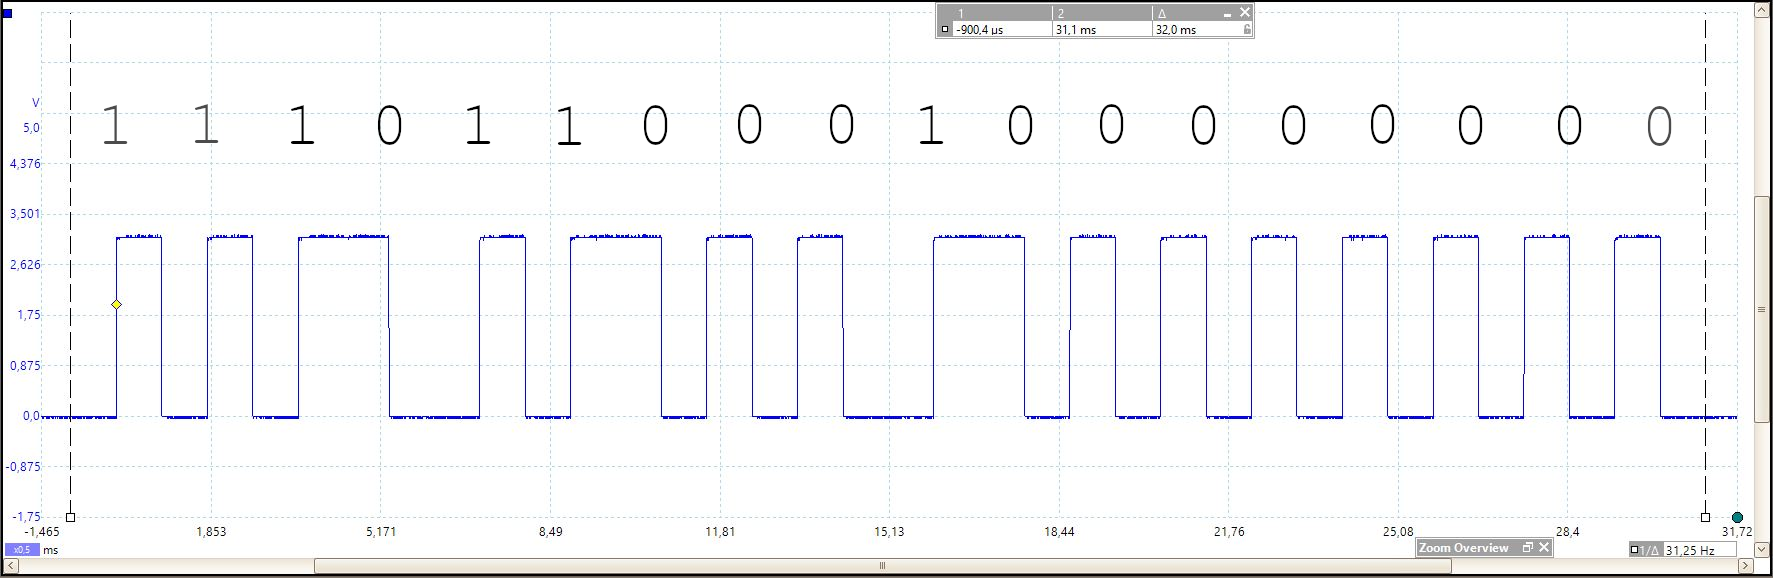
\includegraphics[width=.9\textwidth]{figures/results/manchester/manchester_sequence_141_decoded.png}
	\caption{Manchester Encoded Waveform}
	\label{fig:manchester_sequence_141_decoded}
\end{figure}

The bit period was measured to be 1.777mS, figure \ref{fig:delta_bit_period} in the appendix shows this measurement.


%%%%%%%%%%	DISCUSSION	%%%%%%%%%%
\textbf{Discussion}\\
Inspecting the decoded binary sequence (drawn above the waveform), the two start bits are present followed by the binary for the number 141 (in reverse). The 18\textsubscript{th} bit is a zero, which is the correct parity for the data being transmitted.

The bit period of the waveform matched the expected value of 1.777mS, confirming the functionality of the module and demonstrating the high precision that may be achieved through the use of interrupts and timers.
%%%%%%%%%%	/DISCUSSION	%%%%%%%%%%



%%%%%%%%%%%%%%%%%%%%%%%%%%%%%%%%%%%%%%%%%%%



\subsection{Target MCU Performance}

\subsubsection{Processing Time}

%todo: further crop these pics
\begin{figure}[H]
	\centering
	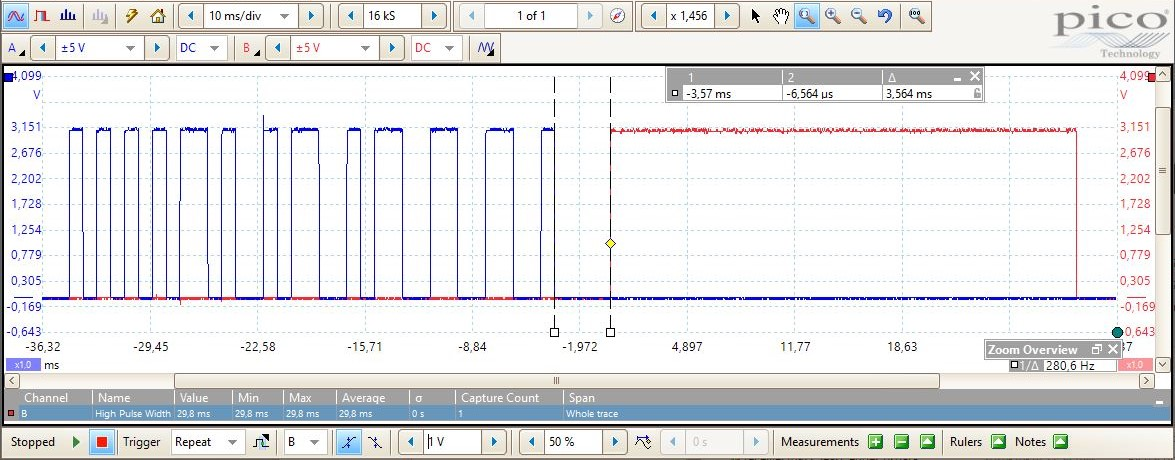
\includegraphics[width=.9\textwidth]{figures/results/receiver_software/arbitrary_11111_timing_test_crop.JPG}
	\caption{Oscilloscope Trace for Transmission of 11111}
	\label{fig:arbitrary_11111_timing_test}
\end{figure}

\begin{table}[H]
	\centering
	\begin{tabular}{cccc}
		\hline
		\textbf{\begin{tabular}[c]{@{}c@{}}15-Bit Data\\ (Decimal)\end{tabular}} & \textbf{Number of Edges} & \textbf{\begin{tabular}[c]{@{}c@{}}Timeout Delay\\ (ms)\end{tabular}} & \textbf{\begin{tabular}[c]{@{}c@{}}Decoding Time\\ (ms)\end{tabular}} \\ \hline
		10922 & 20 & 3.56 & 29.7 \\ \hline
		11111 & 26 & 3.56 & 29.8 \\ \hline
		32767 & 36 & 3.56 & 29.9 \\ \hline
	\end{tabular}
\end{table}

Combining the timeout delay and decoding time gives a maximum period of 33.46ms in the worst case, before a new message may be received.


%%%%%%%%%%	DISCUSSION	%%%%%%%%%%
\textbf{Discussion}\\
%todo: discuss these results
%%%%%%%%%%	/DISCUSSION	%%%%%%%%%%

\subsubsection{Error Handling}
Figure \ref{fig:transmission_too_fast} below shows a set of incoming transmissions (blue trace) that arrive faster than the MCU can process them. Any edges that occur while the MCU is processing a previous message (indicated by the red trace being high) are ignored.

\begin{figure}[H]
	\centering
	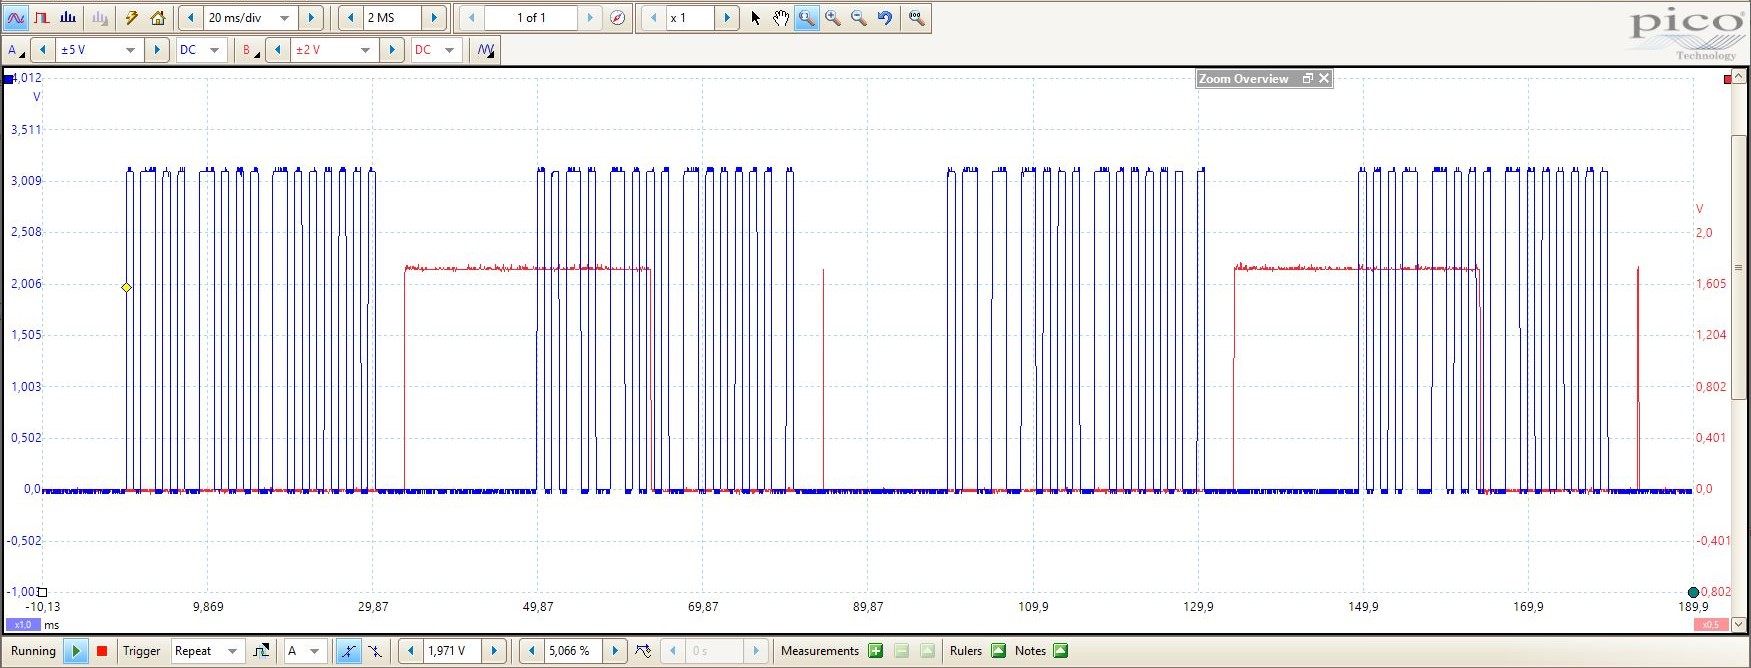
\includegraphics[width=.8\textwidth]{figures/results/receiver_software/transmission_too_fast_crop.JPG}
	\caption{Incoming Transmission During Decoding}
	\label{fig:transmission_too_fast}
\end{figure}

Figure \ref{fig:transmission_too_many_edges} below shows an incoming stream of transmissions with no delay period separating them (blue trace). The time spent processing incoming transmissions is indicated by a high logic level on channel B (red trace).

\begin{figure}[H]
	\centering
	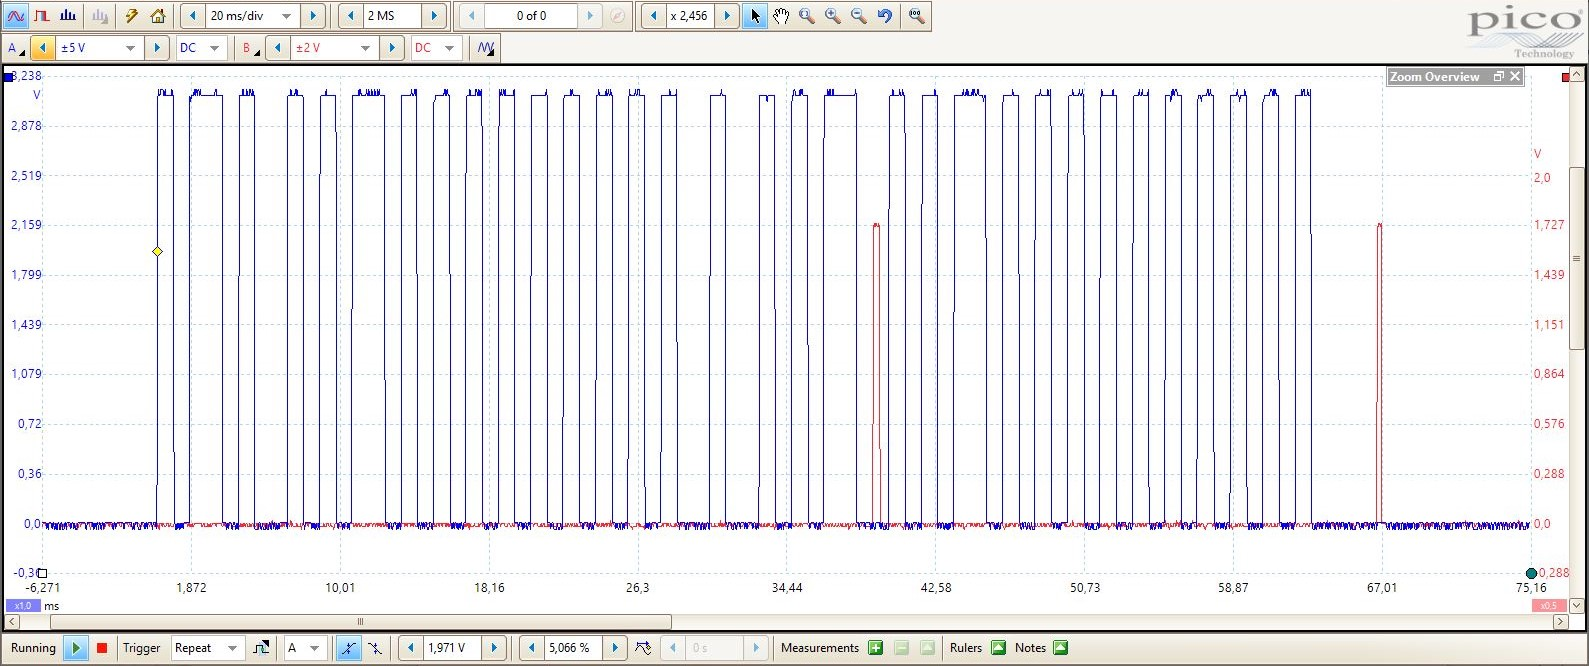
\includegraphics[width=.8\textwidth]{figures/results/receiver_software/transmission_too_many_edges_crop.JPG}
	\caption{Continuous Transmission}
	\label{fig:transmission_too_many_edges}
\end{figure}

%%%%%%%%%%	DISCUSSION	%%%%%%%%%%
\textbf{Discussion}\\
%It seems that the LCD write function is the reson it takes so long to 'process', its not that it is so much drastically longer because its going through all the states.... but its too little too late to change that because soo many experiemnts used that code....
In the case of the two transmissions that arrived while the processor was busy, errors were detected and no further processing was performed. This is indicated by the short red spike that occurs in each case.

In the case of continuous transmission, the maximum number of edges were recorded. When this occurred the processor immediately attempted to decode the transmission. At the point when the processor detected that the number of decoded bits exceeds 18, the message was discarded and no further processing was performed.
%%%%%%%%%%	/DISCUSSION	%%%%%%%%%%




%%%%%%%%%%%%%%%%%%%%%%%%%%%%%%%%%%%%%%%%%%%


%%%%%%%%%%%%%%%%%%%%%%%%%%%%%%%%%%%%%%%%%%%
%%%%%%%%%%%%%%%%%%%%%%%%%%%%%%%%%%%%%%%%%%%

%%%%%%%%%%%%%%%%%%%%%%%%%%%%%%%%%%%%%%%%%%%
%%%%%%%%%%%%%%%%%%%%%%%%%%%%%%%%%%%%%%%%%%%

\section{System Range}

Table \ref{tbl:max_distances_system} below shows the maximum ranges of the system as a consequence of using the different detector modules and the ambient lighting conditions.

\begin{table}[H]
	\centering
	\begin{tabular}{ccc}
		\hline
		Module & \begin{tabular}[c]{@{}c@{}}Maximum Distance\\ Dark Environment\\ (m)\end{tabular} & \begin{tabular}[c]{@{}c@{}}Maximum Distance\\ Bright Environment\\ (m)\end{tabular} \\ \hline
		Phototransistor & 17 & 36 \\ \hline
		Photodiode & 17.5 & SAT \\ \hline
		IR Receiver & 47 \textgreater{} & 47 \textgreater{} \\ \hline
	\end{tabular}
	\caption{Maximum Receiver Distances}
	\label{tbl:max_distances_system}
\end{table}

In a dark environment

\subsubsection{Photodiode Observations}
%todo: this needs description
\begin{figure}[H]
	\centering
	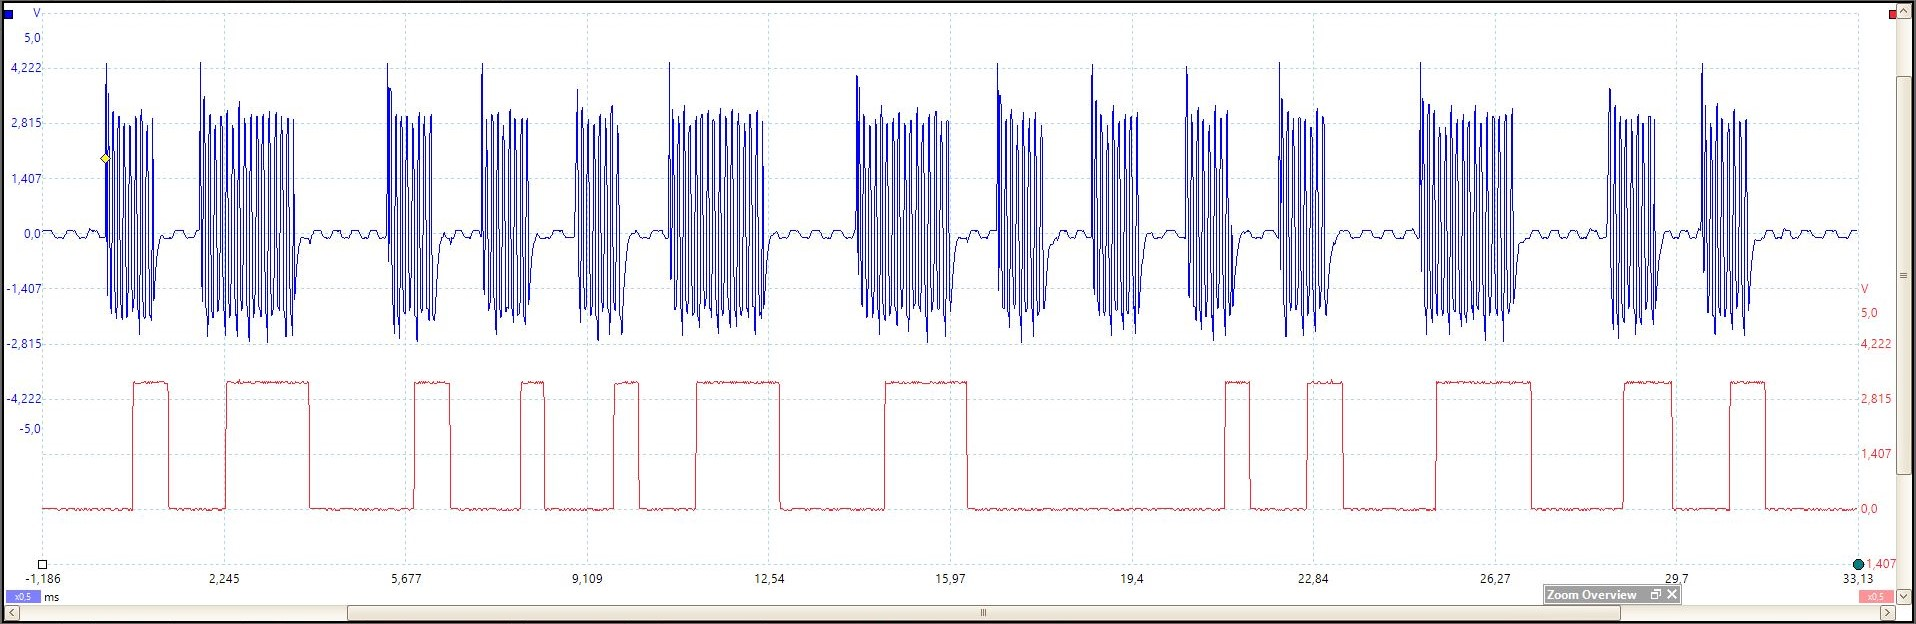
\includegraphics[width=.9\textwidth]{figures/results/drak_system_test/photodiode1750cm_missed_bits.jpg}
	\caption{Oscilloscope trace showing undetected bits at a range of 17.5m - Photodiode Detector in a dark environment}
	\label{fig:photodiode_bit_error}
\end{figure}


\begin{figure}[H]
	\centering
	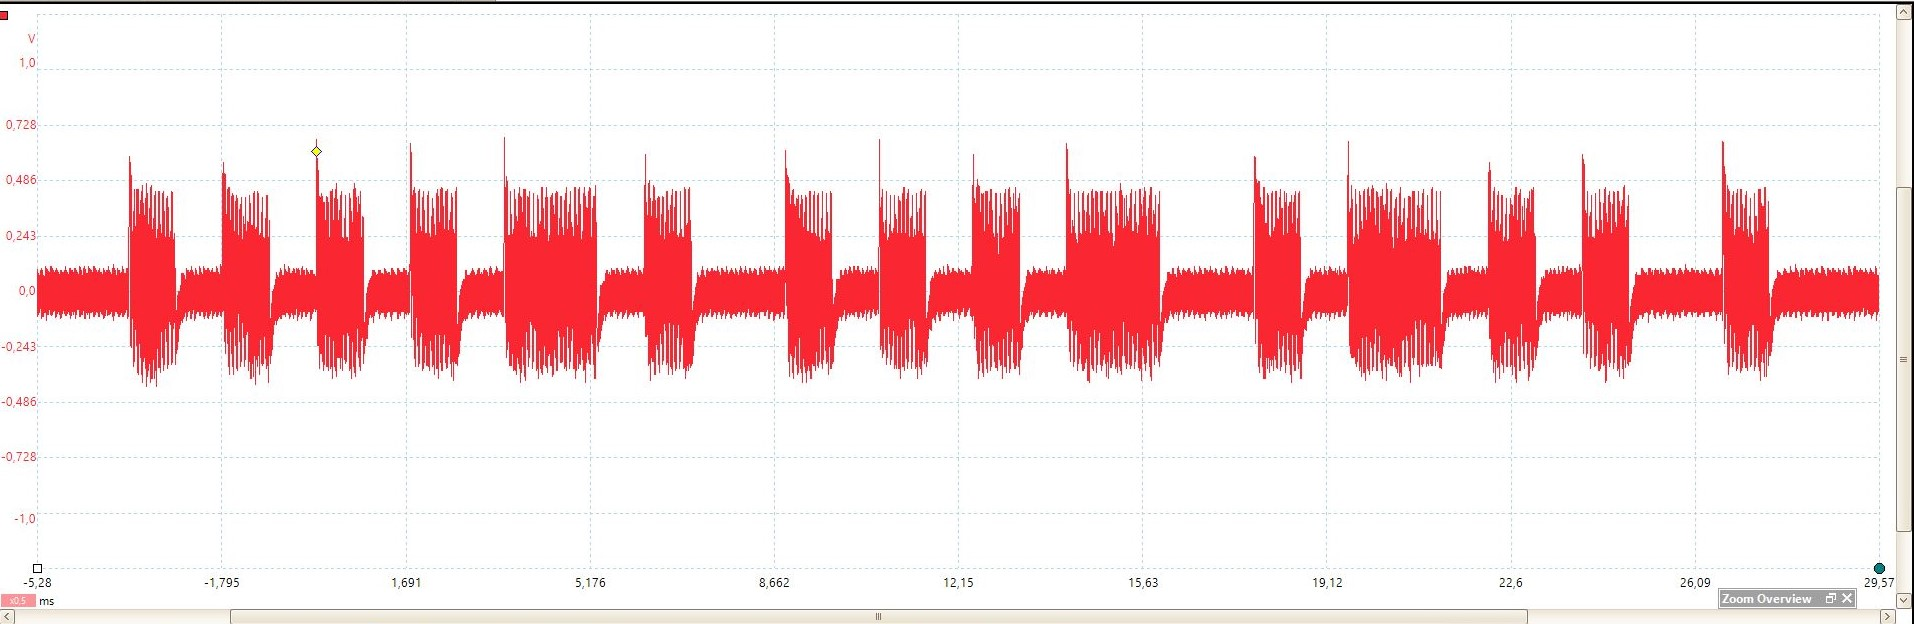
\includegraphics[width=.9\textwidth]{figures/results/drak_system_test/photodiode4770cm.jpg}
	\caption{Oscilloscope trace showing input of Goertzel filter at a range of 47.7m - Photodiode Detector in a dark environment}
	\label{fig:photodiode_range_4770cm}
\end{figure}

\subsubsection{Phototransistor Observations}
%todo: include these images

\begin{figure}[H]
	\centering
%	\includegraphics[width=.9\textwidth]{figures/results/drak_system_test/phototransistor1}
	\caption{Oscilloscope trace showing undetected bits at a range of ?m - Phototransistor Detector in a ? environment}
	\label{fig:phototransistor1}
\end{figure}


\begin{figure}[H]
	\centering
%	\includegraphics[width=.9\textwidth]{figures/results/drak_system_test/phototransistor2}
	\caption{Oscilloscope trace showing input of Goertzel filter at a range of ?m - Phototransistor Detector in a ? environment}
	\label{fig:phototransistor2}
\end{figure}


\subsubsection{IR Receiver Observations}

\begin{figure}[H]
	\centering
	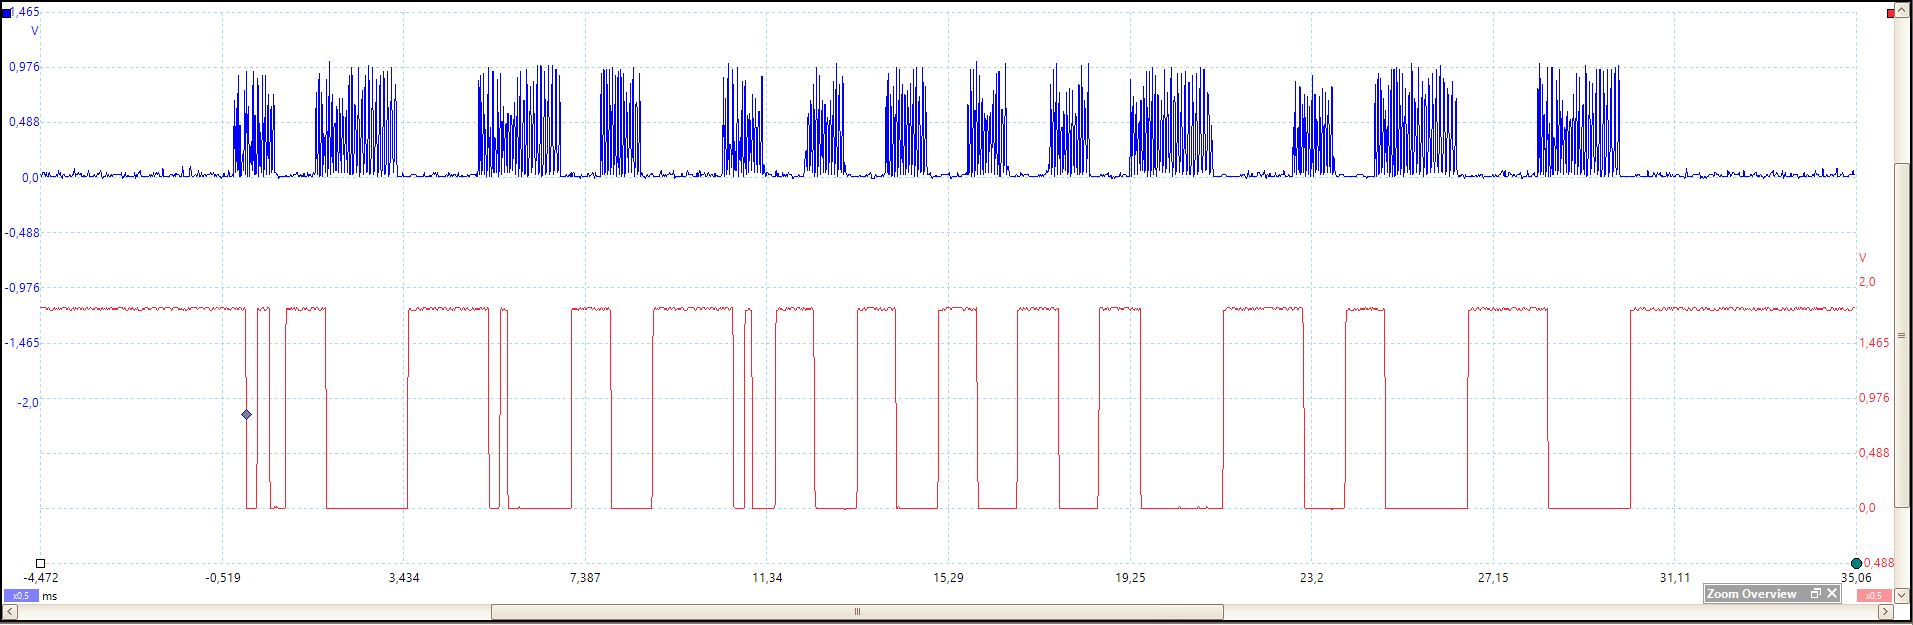
\includegraphics[width=.9\textwidth]{figures/results/system_test/36m_phototranaistoroutput_vs_receiveroutput.JPG}
	\caption{Oscilloscope trace showing the output of the IR receiver and the conditioned output of the phototransistor detector}
	\label{fig:36m_phototranaistoroutput_vs_receiveroutput}
\end{figure}

During the day time range test, it was observed that the output of the IR receiver contained blips. It can be seen in figure \ref{fig:36m_phototranaistoroutput_vs_receiveroutput} that while the incident IR radiation was modulating the output of the IR receiver would occasionally indicate for a brief period that no incident radiation was present. These blips produced errors in the decoded bit-stream.

These blips only presented themselves when the IR receiver was centred in the incoming beam, if the beam was slightly off centre the behaviour ceased.


%%%%%%%%%%	DISCUSSION	%%%%%%%%%%
\textbf{Discussion}\\
%todo: discuss these results
%%%%%%%%%%	/DISCUSSION	%%%%%%%%%%


%%%%%%%%%%%%%%%%%%%%%%%%%%%%%%%%%%%%%%%%%%%
%%%%%%%%%%%%%%%%%%%%%%%%%%%%%%%%%%%%%%%%%%%
